\documentclass[%
reprint,nofootinbib,
amsmath,amssymb,
aps,
]{revtex4-1}
\usepackage{graphicx}% Include figure files
\usepackage{dcolumn}% Align table columns on decimal point
\usepackage{bm}% bold math
\usepackage[utf8]{inputenc}
\usepackage{listings}
\usepackage{amsmath}
\usepackage{physics}
\usepackage{booktabs}
\usepackage{float}
\usepackage[bottom]{footmisc}
\usepackage{scrextend}

\usepackage{caption}
\captionsetup{justification=raggedright,singlelinecheck=false}
\usepackage{subcaption}
\graphicspath{ {./figures/} }




\bgroup
\def\arraystretch{1.3}
\newcommand{\HRule}{\rule{\textwidth}{0.5mm}}
\makeatletter
\newcommand*{\rom}[1]{\expandafter\@slowromancap\romannumeral #1@}
\makeatother

\newcommand{\aegis}[0] {AE$\bar{\textnormal{g}}$IS}
\newcommand{\h}[0] {$\bar{\textnormal{H}}$}



\begin{document}
\onecolumngrid

\begin{center}
	\large\textbf{Modeling the Solar System \\ using ordinary differential equations}
\end{center}
\vspace{5mm}

\begin{center}
	\small{$^1$ Oline A. Ranum}\\
\end{center}

\begin{center}
	\small{$^1$ University of Oslo, Institute of physics, 
		olinear@student.matnat.uio.no}
\end{center}

\begin{center}
	\textit{\today}
\end{center}
\vspace{5mm}
\noindent 
\HRule \vspace{0.1mm}\\
	 This paper presents the results on an attempt to build a model that simulates the planetary orbits in the Solar system, using the forward Euler and velocity Verlet algorithms for ordinary differential equations. A full object oriented implementation is developed for the solar system, and the planetary orbits are propagated according to Newton's gravitational law. A model of Earths orbit around the Sun is used to test the implementation and to perform a sensitivity-stability study of both algorithms. The conservation property of both the energy and angular momentum of Earths motion is evaluated using both algorithms. It is found that the velocity Verlet algorithm is more stable than the forward Euler, and conserve the  orbital properties better. The escape velocity is estimated numerically, and is proposed to be of a value between $v_0\in(8,9)$ AU/yr which corresponds well to the theoretical prediction of $v_0 = 8.886$ AU/yr. The value of the exponent, $\beta = 2$, in Newtons gravitational law is perturbed in a range of values $\beta\in[2,3]$, and it is found that the perturbation distorts the orbit of Earth around the sun to a significant extent. When $\beta \geq 2.7$ we find that Earth is ejected from its orbit, and escapes the solar system. We evaluate the three-three body problem in a Sun-Earth-Jupiter numerical simulation and compare the system when it is orbiting around the Sun fixed in the origin and when all three celestial bodies orbit a common center of mass. We look at the impact Jupiter's presence has on Earths orbit, and the impact of the Jupiter-Sun mass relation on the orbit of Earth. We find that increasing Jupiter's mass causes Earths orbit to become more unstable, and eventually Earth escapes the Solar System. The model is expanded to include all 8 planets of the Solar System, orbiting around a common center of mass. In the end a method is developed for estimating the perihelion precession of Mercury, but it is found that the velocity Verlet algorithm according to the current implementation yields a precision incapable of providing a sensible result at the current stage of the developed code.    
\noindent 
\vspace{1mm}  \\
\HRule
\vspace{0.1cm}


\section{Introduction} 
\twocolumngrid
\noindent Newtons second law, also known the law of gravitation, allows us to describe the orbits of planets and stars using numerical simulation tools. The gravitational interaction dictates how our solar system is formed and evolves, which has been an object of interest for centuries. Modern computational techniques and algorithms such as the velocity Verlet method, has raised the opportunity to better understand the motion of planets by simple simulations. Numerical solvers has become an important tool for understanding the fundamental mechanics of the universe. This paper evaluates the forward Euler and velocity Verlet algorithm to simulate the planetary orbits, and several properties associated with celestial motion. \\ \indent
Initially, this paper presents the central theory for the coupled ordinary differential equations that describes the planetary orbits and basic conserved properties, followed by a brief definition of the algorithms. The second section presents the methods employed to derive the planetary orbits, and the implementation of the algorithms. The planetary system is discretized, and the implementation of the algorithms is tested using the Earth-Sun system. A stability study is performed, and the escape velocity is evaluated numerically and compared to the theoretical expectations. We also look at the effect of increasing the exponent of the distance parameter in Newtons gravitational law on Earths orbit. Thereafter, the system is expanded to include Jupiter and a three-body simulation is performed. The effects of Jupiter's presence on Earths orbit is evaluated, alongside how an increase in Jupiter's mass would impact Earth's trajectory. In the end a full model for all planets of the Solar System is developed, and the orbits are propagated around a common center of mass. A model for evaluating the perihelion precession of Mercury is developed.\\ \indent 
Numerical algorithms allows us to study phenomena which could otherwise be hard to evaluate directly. They yield a new platform for us to understand the implications of the models we construct to describe extraterrestrial mechanics. It is our hope that this paper will be a contribution for a better understanding of the limitations and opportunities presented by numerical algorithms in combination with the employment of physical models. 
\newpage

\onecolumngrid 

\section{Theory} \vspace{5mm}

\twocolumngrid 

\noindent 
This section provides an introduction to the basics of Newton's gravitational law and the ordinary differential equations that describe the motion of planets. Some central properties are introduced, such as the escape velocity and the perihelion precession of Mercury. The algorithms that will be employed to solve the differential equations for the solar system simulation, the forward Euler and velocity Verlet method, is briefly described. \\

\subsection{Newton's law of gravitation} \noindent 
The Newtonian law of gravitation states that the gravitational interaction between an object $i$ and and an object $j$ can be described as a force $F_G$, where \vspace{3mm}\\
\begin{equation}\label{nwt}
	\vec{F}_G = \frac{GM_iM_j}{r_{ij}^2}\hat{r}_{ij} = \frac{M_jv_j^2}{r_{ij}}\hat{r}_{ij}
\end{equation} \vspace{3mm} \\
where $M_i$ is the mass of object $i$, $M_j$ is the mass of object $j$, $G=4\pi^2$ is the gravitational constant in astronomical units, $r_{ij} = \sqrt{x^2+y^2+z^2}$ is the distance between object $i$ and $j$ and $v_j$ is the velocity of object $j$. In the case of the Sun-Earth system, this implies that the following velocity relation should hold\vspace{5mm} \\
\begin{equation}\label{motion1}
	v_{E}^2r_{E, \odot} = GM_{\odot} = 4\pi^2\dfrac{(\textnormal{AU})^3}{(\textnormal{yr})^2}
\end{equation}\vspace{5mm}\\
where $M_{\odot}$ is the mass of the Sun, $v_{E}$ is the velocity of earth and $r_{E,\odot}$ is the distance between the earth and the sun. By rearranging the parameters of equation \ref{nwt} it is possible to define the following equation of motion for a two-body system\vspace{3mm}\\ 
\begin{equation}\label{mot2}
	\dfrac{d^2r_i}{dt^2}=\dfrac{F_{G,r_i}}{M_{\mathrm{Earth}}}
\end{equation}\vspace{3mm} \\ 
where $F_{G,r_i}$ is the component of the gravitational force along dimension $i$.
A circular motion is produced when the initial velocity is approximately given by \vspace{3mm}\\
\begin{equation}\label{v0}
	v_0 \approx \sqrt{\dfrac{GM_\odot}{r}}
\end{equation} \newpage \noindent 
It is well known that Newton's gravitational law describes a conservative force. That is, a force who conserves the total energy of the system in the case that there are no external forces performing a work on the environment. In the case of a celestial object in orbit around another object, the total energy $E_{tot}$ can be described as the sum of the kinetic energy $E_k$ and potential energy $E_p$, respectively \vspace{3mm}  \\ 
\begin{align}
	E_k &= \dfrac{1}{2}M_jv_j^2 \label{Ek}\\ 
	& \nonumber \\ 
	E_p &= -G\dfrac{M_iM_j}{r_{ij}} \label{Ep}
\end{align} \vspace{3mm}  \\
It follows that the total mechanical energy for a N body system is given by the sum of the energy components for each object $j$ in the system \vspace{3mm} \\ 
\begin{equation} \label{Et}
	E_{tot} = E_k + E_p =  \sum_{j = 0}^{N} \dfrac{1}{2}M_jv_j^2 - G \sum_{j<i}\sum_{i}^{N} \dfrac{M_iM_j}{r_{ij}}
\end{equation}  \vspace{3mm} \\ 
where $N$ represents the number of planets. Furthermore, the gravitational force conserves the angular momentum of an isolated system  \vspace{3mm} \\ 
\begin{equation}\label{lmomentum}
	\vec{l} = \sum_{j}^{N}\vec{r}_j\cross \vec{v}_j
\end{equation}  \vspace{3mm} \\ 
The quantities are conserved due to the absence of any external forces or torque [M. Jensen, 2015]. 

\subsection{Escape velocity} \noindent 
The escape velocity of an object is the velocity necessary for a body to escape a gravitational potential, and this velocity is reached once the kinetic energy becomes larger than the potential energy. By using the law of energy conservation and equation $E_k$ and $E_p$ it is possible to derive the following expression for the escape velocity  \vspace{3mm} \\
\begin{equation}\label{vesc}
v_{esc} = \sqrt{\dfrac{2GM_\odot}{R}} = \sqrt{2}v_0
\end{equation} \vspace{3mm} \\
For the Earth-Sun system with $G = 4\pi^2$ and $M_\odot = 1$ the escape velocity is equal to $v_{esc} = 8.886$ AU/yr [M. Jensen].

\subsection{The perihelion precession of Mercury} \noindent 
The observed value for the perihelion precession of Mercury, when all classical effects are subtracted is 43$^{''}$ per century. There is a number of reasons why the perihelia of planets precess in orbit around stellar objects, but in general one sees that any correction to the pure $r^{-2}$ behavior of Newton's gravitational law causes objects in orbit to shift slightly after a full period. The general relativistic correction to the Newtonian gravitational force between the Sun and Mercury can be described as \vspace{3mm} \\
\begin{equation}
	F_G = \dfrac{GMM_{\odot}M_{Merc}}{r^2}\qty[1 + \dfrac{3l^2}{r^2c^2}]
\end{equation}  \vspace{3mm} \\
where $M_{Merc}$ is the mass of Mercury, $r$ is the distance between Mercury and the sun, $l = \abs{\vec{r}\times \vec{v}}$ is the magnitude of Mercury's orbital angular momentum per unit mass, and $c$ is the speed of light in vacuum. The perihelion angle $\theta_P$ is given by\\
\begin{equation}\label{per}
	\tan{\theta_P} = \dfrac{y_P}{x_P}
\end{equation} \\ 
where $x_P(y_P)$ is the $x(y)$ position of Mercury at perihelion, i.e. at the point where Mercury is at its closest to the Sun [M. Jensen].

\subsection{Numerical Solvers} \noindent 
The above differential equations are solvable using numerical estimation techniques.  
The forward Euler method is a unsymmetrical first order differential solver algorithm that advances a solution on an interval $h$, using the derivative information at solely the beginning of the current interval. This indicates that the error of each step is proportional to $h$. Euler's method is in general not recommended for practical use at it is considered to be inaccurate and unstable solver [Press et al., 2007]. Euler's method is derived using a Taylor approximation on the slope of a function $f$ over an interval h \vspace{3mm} \\ 
\begin{equation}
		\dfrac{df}{du} = \lim_{u\to\infty} \dfrac{f(u+h) -f(u)}{h}
\end{equation} \\ 
implying that \\ 
\begin{equation}
	\dfrac{df}{du} \approx \dfrac{f(u+h) -f(u)}{h}
\end{equation} \vspace{3mm} \\ 
It follows that \vspace{3mm}\\
\begin{equation}
	f(u+h) \approx f(u) + h\dfrac{df}{du}
\end{equation} \vspace{3mm}\\ 
Taking in to consideration the error of performing the above approximation, the forward Euler scheme can be completely described as\vspace{3mm} \\ 
\begin{equation}\label{euler1}
	u(t + h) = u(t) + hu^{(1)}(t) + \order{h}
\end{equation} 
\begin{equation}\label{euler2}
	u^{(1)}(t+h) = u^{(1)}(t) + hu^{(2)}(t) + \order{h}
\end{equation}\vspace{3mm} \\
where $u^{n}$ is the $n$th derivative of $u$. \\  \indent 
The velocity Verlet algorithm is numerically stable, and is thus considered to be more reliable than Euler's forward algorithm. The Verlet method is based on a Taylor expansion as well, but to the second order so that \vspace{3mm} \\
\begin{equation*}
u(t+h) = u(t) + hu^{(1)}(t) + \dfrac{h^2}{2}u^{(2)}(t)) + \order{h^3}
\end{equation*} 
\begin{equation*}
u^{(1)}(t+h) = u^{(1)}(t) + hu^{(2)}(t) + \dfrac{h^2}{2}u^{(3)}(t)) + \order{h^3}
\end{equation*} \vspace{3mm} \\ 
In order to remove the third derivative the following approximation can be employed \vspace{3mm} \\ 
\begin{equation}\label{sub}
	u^{(3)}(t) = \dfrac{u^{(2)}(t + h) +u^{(2)}(t)}{h}
\end{equation} \vspace{3mm}\\ 
when inserting equation \ref{sub} in to the Taylor approximation equations one obtains the following relations\vspace{3mm} \\ 
\begin{align}\label{vv1}
	u(t+h) = u(t) + h\qty(u^{(1)}(t) + \dfrac{h}{2}u^{(2)}(t)) + \order{h^3} \nonumber \\ 
\end{align} 
\begin{align}\label{vv2}
	u^{(1)}(t+h) = u^{(1)}(t) + \dfrac{h}{2}\qty(u^{(2)}(t + h)+u^{(2)}(t))  + \order{h^3} \nonumber \\ 
\end{align}

\onecolumngrid

\section{Method}
 \vspace{5mm}
 
\twocolumngrid 
 \noindent 

\subsection{Building a simulation framework}\noindent
In order to build a model for planetary orbits we develop an object oriented code, which employs the forward Euler and velocity Verlet algorithms to solve for the coupled second order differential equations described by equation \ref{nwt} in three dimensions. A general class \textit{SolarSystem} is developed which takes planetary properties as input values. In regards to the input an instance of the class \textit{Planets} is created for each planetary object. \\ \indent The class \textit{ODESolver} is then called in order to solve the coupled equations described by relation \ref{mot2}. The \textit{ODESolver} class has three methods. One method employing the forward Euler algorithm, and two methods employing the velocity Verlet algorithm. The first Verlet method solves a two-body system, which is generalized into the second Verlet method who solves an N-body system. The forward Euler solver is based on equation \ref{euler1} and \ref{euler2}, and is implemented in the following manner\\ 
\begin{align}
	\vec{v}_i & = \vec{v}_{i-1} + h\vec{a}_i & \hspace{2mm} i \in {1, 2, ..., N} \nonumber\\ 
	\vec{x}_i & = \vec{x}_{i-1} + h\vec{v}_i & \hspace{2mm} i \in {1, 2, ..., N}\nonumber
\end{align} \\ 
The acceleration is vectorized and estimated as given by equation \ref{nwt}. The velocity Verlet procedure is implemented based on equation \ref{vv1} and \ref{vv2}, and is employed as follows \\ 
\begin{align}
	\vec{v}_i &= \vec{v}_{i-1} + \dfrac{h}{2}(\vec{a}_i + \vec{a}_{i-1}) & \hspace{2mm} i \in {1, 2, ..., N} \nonumber\\ 
	\vec{x}_i &= \vec{x}_{i-1} + h\vec{v}_{i-1} + \dfrac{h^2}{2}\vec{a}_{i-1} & \hspace{2mm} i \in {1, 2, ..., N} \nonumber
\end{align} \\ 
It is initially assumed that the motion of the Sun can be neglected, as the mass of the Sun is significantly larger than the mass of the Earth. Equation \ref{motion1} is discretized on a finite time axis $t\in[t_0, t_{f}]$ of N points, implying a resolution $h = (t_f-t_0)/N$. It follows that the position and velocities evaluated in time is discretized so that $r_i = r(t_i)$ and $v_i = v(t_i)$ in every spatial dimension $i$, propagated based on an acceleration $a_{i} = a(r_i)$. \\ \indent 
\subsection{Test of implementation and stability} \noindent
In order to test the implementation we employ the solver to propagate Earths orbit around the Sun. The gravitational constant is scaled to $G = 4\pi^2$ and the mass of the Sun to $M_\odot = 1$. The masses of all other planets are scaled in regards to the mass of the Sun. The Sun is initiated in the origin where it will remain fixed for the initial simulations, and Earth is initiated in a position $r_0 = [1, 0, 0]$ AU. To produce roughly circular orbits the system is initiated using equation \ref{v0} to set the initial velocity. The velocity $v_0$ is derived from this initial condition and distributed equally in the $y$ and $z$ spatial dimension. Both algorithms are employed to propagate the simulation. \\ \indent 
The numerical stability of both algorithms are tested by varying the number of integration points $N$. The trajectory of Earth orbiting the sun is evaluated for $dt = 10^{-i}$ with $i\in{2,3,4}$ over a period of 10 years. \\ \indent 
A further evaluation of the solver's stabilities is performed by evaluating the conservation of energy in the system as a function of time using equation \ref{Ek}, \ref{Ep} and \ref{Et}. Conservation of angular momentum is also tested over time using equation \ref{lmomentum}. An evaluation is performed on which algorithms preserves the quantities that should be conserved. \\ \indent 
A timing is performed for both algorithms, and the number of floating point operations necessary to perform the simulation is counted. The time estimates are provided as the average of 10 independent test runs, with the error estimate being the standard deviations between the individual test times. The velocity Verlet algorithm are employed for the remainder of this project. \\ 

\subsection*{Estimating the escape velocity} \noindent 
The implementation is then employed to give an estimate of the escape velocity of Earth in a bound orbit around the sun. Earth is given an initial distance of 1 AU from the sun on the x-axis, and the test is performed by trail and error. The initial velocity is equally distributed on the y- and z-axis, and tested for a range of values $v_0\in\{2,4,6,8,9,10\}$ AU/yr.  The simulations are performed using $N=10^7$ points over a period of 10 years. The numerical results are compared with the expected analytical solution of equation \ref{vesc}. \\ \indent 
Following the test of the initial velocity, an evaluation is performed on the impact of perturbing the the exponential value $\beta$ of $r$ in equation \ref{nwt}. The value of  $\beta$ is varied within a range $\beta \in [2.0, 3.0]$, using a step size of $\Delta \beta = 0.1$. 

\subsection*{The three-body problem} \noindent
The next section considers the numerical evaluation of a three-body system. The Sun-Earth system is expanded to include Jupiter, still while keeping the Sun fixed at the center of the system. The orbits of Earth and Jupiter is first evaluated keeping Jupiter's mass at it's actual ratio to the mass of the Sun. The impact of Jupiter presence on Earths orbit is evaluated by adding the force between Jupiter and Earth as dictated by equation \ref{nwt} to the acceleration of Earth. The simulation is performed using $N=10^7$ points over a period of 10 years. The initial conditions is now set to be equal to initial conditions as recorded by NASA for the 15th of November 2019. A full list of the initial conditions of all planets can be found in the appendix. A stability study is performed on the orbit of earth under the impact of Jupiter's presence, using the Verlet solver. \\ \indent 
A study is performed on how the Jupiter-Sun mass ratio affects the orbit of earth. Jupiter's mass is first increased by a factor of 10, and then by a factor of 1000. The stability of Earth's orbit is reevaluated for both mass ratios.
 
\subsection*{Three-body simulation} \noindent
A real three-body calculation is then performed by setting the Sun in motion, and placing the origin in the center of mass. The relocation of the origin to the center of mass is performed by giving the Sun an initial velocity which makes the total momentum of the system exactly zero. Earths, Jupiter's and the Suns orbit are recalculated, and compared to the results of the three-body simulation where the Sun was fixed at the origin.  \\ 

\newpage

\subsection*{A Solar System N-body simulation} \noindent 
The remaining planets of the solar system is added and every orbit is propagated taking the impact on the acceleration from the other planets into consideration. The simulation is still performed using $N=10^7$ points but the period is extended to a period of 200 years. The initial conditions on position and velocities are obtained from the NASA database, as described in the appendix. 
\subsection*{The perihelion precession of Mercury} \noindent 
The system developed is then employed to predict the perihelion precession of Mercury. Holding the sun fixed in the origin, the orbit of mercury is initiated in perihelion at $x = 0.3075$ AU with an initial velocity $v_y = 12.44$ AU/yr. The orbit is propagated for a period of 100 years. Then the distance $r$ from the Sun is evaluated at every time step, and for each orbit the minimum distance $r_{perihelion}$ is located. At this point the angle $\theta_P$ is estimated using equation \ref{per}. Plotting the evolution of $\theta_P$ for each full orbit over a century should indicate a drift in the angular value. Using a linear fit across the data, and then taking the final angle and subtracting the initial angle should yield an estimate of the perihelion precession of Mercury per century. \\ 

\onecolumngrid

\vspace{15mm}

\section{Results} 
\vspace{5mm}

\begin{figure}[H]
	\includegraphics[scale = 0.15]{Figures/A103.png} \hspace{5mm}
	\includegraphics[scale = 0.15]{Figures/A104.png} \hspace{5mm}
	\includegraphics[scale = 0.15]{Figures/A105.png}
	\caption{\textit{The orbit of Earth propagating around the sun (yellow) using the Forward-Euler (blue) and the velocity Verlet (red) algorithms for N = $10^i$ with $i\in{3,4,5}$ time steps for 10 years,  yielding time steps $dt = 10^{-i}$ with $i\in{2,3,4}$. The Verlet algorithm has a stable performance in every case, the Euler algorithm is on the other hand unstable and quickly propagates away from the supposed orbit for low time resolutions. The stability of the Euler algorithm increases at $dt$ decreases. The initial condition is set as $x_0 = 1, y_0 = 0, z_0 = 0$, $ v_x = 0, v_y = v_0/\sqrt{(2)}$, $ v_z = v_0/\sqrt{2}$, where $v_0$ is given by equation \ref{v0}, $G = 4\pi^2$ and $M_\odot = 1$.} \label{earthsun}}
\end{figure}

\vspace{15mm}

\twocolumngrid

\noindent 
Figure \ref{earthsun} shows the propagated tracks of the Earth-Sun system while using both the Forward-Euler and the velocity Verlet algorithm for the time steps $dt = 10^{-2}$, $dt = 10^{-3}$ and $dt = 10^{-4}$ . For $dt = 10^{-2}$ it is clear that the forward Euler algorithm is highly unstable, and rapidly spirals outwards and away from the Sun. The velocity Verlet algorithm appears on the other hand to provide a stable track for the temporal resolution $dt = 10^{-2}$. As the value of $dt$ decreases, it is evident that the forward Euler algorithm converges towards a more stable orbit. At $dt = 10^{-4}$ there is visually no difference between the orbits propagated by forward Euler and the velocity Verlet solver. In general, the stability tends to increase as the temporal resolution increases and $dt$ becomes smaller. \\ \indent 
The kinetic, potential and total energy of the Sun-Earth system using both algorithms are plotted in figure \ref{energy} for $N = 10^5$. It is evident that the energy and angular momentum are conserved by the Verlet algorithm. The total energy is found to be constant, within a small distribution fluctuating in the order of $10^{-6}$ for the Verlet algorithm. On the other hand, it is evident that the quantities have a drifting amplitude, and is therefore not conserved when the Euler algorithm is applied. \\
\begin{equation*}
	t_{Euler} = 0.299 \pm 0.006 \textnormal{ s}
\end{equation*}
\begin{equation*}
t_{Verlet} =0.314 \pm 0.009 \textnormal{ s}
\end{equation*} \\ 
\begin{equation*}
	FLOPS_{Euler} = 28N
\end{equation*}
\begin{equation*}
FLOPS_{Verlet} = 49N
\end{equation*}\\ 
\noindent 
When employing the Verlet algorithm to search for the escape velocity one finds that the escape velocity is somewhere in between 8 and 9 AU/yr. That is, the orbit produced using $v_0 = 8$ AU/yr is still a closed orbit, but for $v_0 = 9$ AU/yr it is clear that the orbit is no longer closed and Earth is ejected from its' path around the Sun. The evaluations of the escape velocity is plotted in figure \ref{escape}. Until the escape velocity is reached, an increase of the initial velocity solely causes the major and minor axis to increase. It is evident that the numerical evaluations coincide well with the theoretical expectation of $v_0 = 8.886$ AU/yr. \\ 
\indent  When looking at the effects of varying the $\beta$-parameter there is evidently two kinds of implications. For $\beta = 2$ we get the expected bound circular orbit. For $\beta\in[2.1, 2.6]$ the orbit is still bound, but highly unstable. The orbit appears to become slimmer as $\beta$ increases. For $\beta\in[2.7, 3.0]$ the trajectory is no longer bound to its orbit, and Earth escapes the solar system with a velocity increasing proportional to $\beta$. In general, as $\beta$ increases Earth gets dragged closer towards the Sun, where it appears to accelerate increasingly until Earth is ejected out of the solar system.\\ \indent 
\begin{figure}[H]
	\includegraphics[width = \columnwidth]{Figures/EC.png}
	\vspace{3mm}
	\caption{\label{energy} \textit{Amplitude of energy and angular momentum through the orbit propagations using velocity Verlet (upper) and forward Euler (Lower), for a period of 10 years with $N = 10^5$ integration points. The velocity Verlet algorithm appears to conserve both the energy and angular momentum, with minimal drift for the evaluated period. The forward Euler algorithm has a clear drift the the amplitudes of the values, and both the energy and angular momentum appears to diverge over time. }}
\end{figure}
\vspace{0.1cm}
\begin{figure}[H]
	\includegraphics[width = \columnwidth]{Figures/Escape.png}
	\caption{\label{escape} \textit{The orbits of Earth revolving the Sun, with perturbations of the initial velocity. The escape velocity of Earth from the Sun's gravitational field is indicated by en end of the sequence of closed orbits. Earth appears to have a closed orbit for $v_0=8$ AU/yr, while Earth appears to escape the orbit for $v_0 = 9$ AU/yr. This coincides well with the theoretical predication of Earths escape velocity on $v_0 = 8.886$ AU/yr.}}
\end{figure}

\onecolumngrid

\newpage


\begin{figure}[H]
	\centering 
	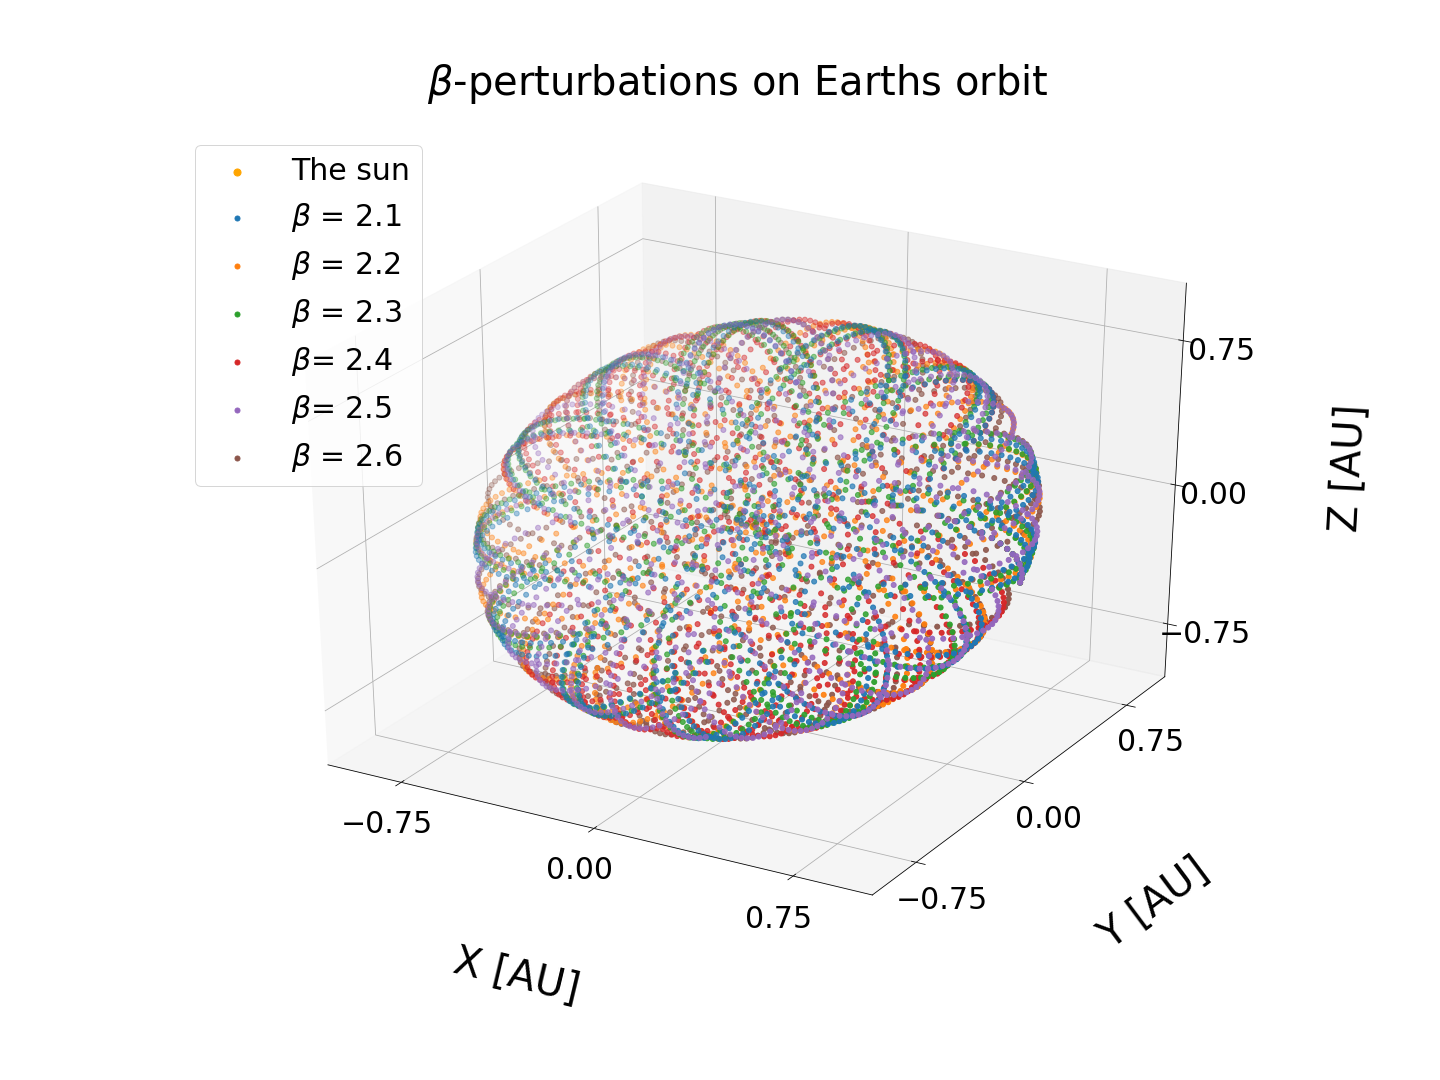
\includegraphics[width = 0.45\columnwidth]{Figures/betta2.png}
	\includegraphics[width = 0.45\columnwidth]{Figures/betta3.png}
	\caption{\label{betta2} \textit{a. The implications of increasing the $\beta$-parameter on Earths orbit, where $\beta\in[2.1, 2.6]$. It is apparent that alternating the $\beta$-parameter in this range yields an unstable, but bound orbit. The orbital paths appears to become slimmer as $\beta$ increases. b. The implications of increasing the $\beta$-parameter on Earths orbit, where $\beta\in[2.7, 3.0]$. It is apparent that alternating the $\beta$-parameter in this range causes the Earth to escape the Suns' gravitational field. }}
	\vspace{10mm}
\end{figure} 

\twocolumngrid

\noindent Figure \ref{threebody} shows the trajectories of Earth around the Sun, kept fixed at the origin, in regards to the perturbations to Earths orbit caused by the presence of Jupiter. The system with both Earths' and Jupiter's' orbit around the origin and Sun is plotted in figure \ref{threebody}\textit{a}, where it appears that Earth's orbit is rather stable. Figure \ref{threebody}.\textit{b} shows how Jupiter's presence impact the orbit of Earth closer up. It is evident that Earths orbit is affected by Jupiter's motion, and that Earths orbit becomes more unstable over time. One can see that Earths orbit slightly shifts every year. Figure \ref{threebody}.\textit{c} shows what happens to Earths orbit if Jupiter's mass had been 10 times the amount of what it is estimated to be. It is evident that this increase in mass causes Earths orbit to become even more unstable. Figure \ref{threebody}.\textit{d} shows how Earths orbit would have looked if Jupiter had a mass roughly equal to the mass of the Sun. It is evident that Earth would have been ejected out of orbit, and emitted out of the solar system. \\ \indent

\onecolumngrid


\begin{figure*}[t!]
	\centering
	\begin{subfigure}{0.45\textwidth}
		\centering
		\includegraphics[width = \columnwidth]{Figures/SEJ_NormalMass.png}
		\caption{\textit{The orbit of Earth and Jupiter revolving the Sun. }}
	\end{subfigure}%
	~ 
	\begin{subfigure}{0.45\textwidth}
		\centering
		\includegraphics[width = \columnwidth]{Figures/SEJ_Part1.png}
		\caption{\textit{The orbit of Earth around the Sun with and without the presence of Jupiter. Jupiter causes the orbit of Earth to become more unstable}}
	\end{subfigure}\\ 
	\begin{subfigure}{0.45\textwidth}
		\centering
		\includegraphics[width = \columnwidth]{Figures/SEJ_Part2.png}
		\caption{\textit{The orbit of Earth around the Sun under the impact of Jupiter's presence, when Jupiter's mass is increased to 10 times the actual amount. Jupiter is now 1\% the mass of the Sun. It is evident that the orbit has grown even more unstable.}}
	\end{subfigure}
	\begin{subfigure}{0.45\textwidth}
		\centering
		\includegraphics[width = \columnwidth]{Figures/SEJ_Part3.png}
		\caption{\textit{The orbit of Earth around the Sun under the impact of Jupiter's presence, when Jupiter's mass is increased to 10 times the actual amount. Jupiter is approximately the mass of the Sun. As following, Jupiter causes earth to accelerate and escape the Solar system entirely.}}
	\end{subfigure} \vspace{1mm}
	\caption{\textit{The orbit of Earth around the Sun, kept fixed at the origin, and the impacts of the presence of Jupiter. The propagations are evaluated over a period of 10 years, with a temporal resolution $dt = 10^{-4}$.} \label{threebody}}
\end{figure*}

\begin{figure}[H]
	\includegraphics[width = 0.32\columnwidth]{Figures/Comparing_Sun.png} \hspace{2mm}
	\includegraphics[width = 0.32\columnwidth]{Figures/Comparing_Sun_Earth.png} \hspace{2mm}
	\includegraphics[width = 0.32\columnwidth]{Figures/Comparing_Jupiter.png}
	\caption{\label{ThreeBody} \textit{Comparison of orbits while performing a three body simulation with a). The planets orbiting the Sun kept fixed in the origin and b). The planets and the Sun orbiting a common center off mass. In the right-most figure it is evident that the Sun starts to orbit the origin with a small radius, equally as the planets, in the center of mass system. The middle figure shows how small fluctuations in the position of the Sun causes additional motion in the orbit of Earth. In the figure to the left one can see the track of Jupiter, the orbit is only slightly perturbed if anything.}}
\end{figure}

\newpage 

\twocolumngrid

\noindent 
In figure \ref{ThreeBody} the orbit of the Sun, Earth and Jupiter orbiting a common center of mass and the sun kept fixed in the origin is compared. It is evident that allowing the Sun to orbit a center of mass causes slight perturbations in the trajectory of Earth. There are also slight perturbations in the track of Jupiter, although not visibly representable according to the order of magnitude of the perturbations. \\ \indent 
Figure \ref{SolarSystem} shows the orbits of every planet in the Solar System under the presence of all other planets, orbiting around a common center of mass. The right hand side of figure 7 shows a close up of the inner Solar System in order to give a higher visual resolution of the inner orbits. \\  \indent 
At the end of this project, an attempt was made at estimating the perihelion precession of Mercury. The results of the attempt is presented in figure \ref{Merc}, yielding a precession of approximately 3000$^{''}$. This estimate is roughly 70 times larger than the expected result of 43$^{''}$. Looking at the left-most plot of figure 7 it is evident that Mercury's orbit is rather unstable. It appears that the method applied to locate the perihelion was successful, but that the resolution and numerical stability of the orbital calculations were to poor to yield a sufficient signal. The central plot of figure 8 shows the estimations of $r$ for the first year around, orbiting around the Sun. It is evident that the minimum point of the periodic curve should yield $\theta_P$. The right hand side of figure 7 shows the attempt at employing the estimated $\theta_P$ values to derive the perihelion precession. 

\onecolumngrid

\newpage 

\vspace{2cm}

\begin{figure}[H]
	\includegraphics[width = 0.5\columnwidth]{Figures/5FFullSystem.png} 
	\includegraphics[width = 0.5\columnwidth]{Figures/5FFullSystem_inner.png} \vspace{5mm}
	\caption{\label{SolarSystem} \textit{A full simulation of the solar system around a common center of mass. The right hand figure shows the tracks off all planets in the solar system in three dimensions. The left hand figure shows a close up of the right hand figure, illustrating the orbits of the inner solar system. The simulation is performed over 200 Earth years with $N = 10^7$ integration points, using a velocity Verlet solver.}}
\end{figure}

\vspace{2cm}

\begin{figure}[H]
	\includegraphics[width = 0.32\columnwidth]{Figures/perhielionper1.png} \hspace{2mm}
	\includegraphics[width = 0.32\columnwidth]{Figures/perhielionper2.png} \hspace{2mm}
	\includegraphics[width = 0.32\columnwidth]{Figures/perhielionper3.png}
	\vspace{5mm}
	\caption{\label{Merc} \textit{Results of the attempt to approach an estimate of the perihelion precession of Mercury. The right hand figure shows the orbit of Mercury around the Sun over a period of 100 years, using $N = 10^8$ points. There is evidently some instability trends in the orbit. The middle figure shows a plot of the absolute value of the position, $r$ (blue line), of Mercury around the sun. The perihelion, or the position of Mercury closest to the sun is represented equal to the local minimum values (red dots) of the periodic curve. The right hand figure shows the displacement of $\theta_P$ (red dots) over a century. There is a consistency in the displacement, but the data appears to be to noisy with a to low stability to produce any meaningful result}}
\end{figure}

\newpage 

\twocolumngrid 

\section{Discussion} \noindent 
It was found that velocity Verlet consistently produced more stable tracks relative to the forward Euler approach This is as expected, due to the nature of the numerical stability of the two methods. Forward Euler is asymmetric in time, since it employs information of the derivative only from the first point of the current time interval. Furthermore, it is easy for the Euler method to encounter instability issues as the position and velocity is stored separately, and thus can become numerically unsynchronized. The velocity Verlet algorithm, on the other hand, takes both the current and previous position and velocity estimates into account. The algorithm is numerically stable, and integrates the velocity only in the final step. Therefore, the Verlet algorithm does not suffer from the same instability issues as forward Euler [M. Jensen].\\ \indent 
As is expected according to the theory of conservative fields, the solver methods applied should in principle conserve both energy and angular momentum. However, when employing the forward Euler method it is observed that the energy diverges over time. This is a typical feature of non-time reversible algorithms, and one of the main reasons why the forward Euler algorithm is considered to be unreliable and do not exhibit area-preservation The velocity Verlet algorithm is on the other hand expected to conserve energy and momentum in the limit of $\Delta t \rightarrow 0$ [M. Jensen]. In practice there should be a small energy drift, but as observed by the results this appears to be negligible in regards to the forward Euler estimates]. \\ \indent 
It is evident that the velocity Verlet algorithm is somewhat more time consuming than the forward Euler algorithm. This is expected as the velocity Verlet is a second order estimation, and thus should need more float points operations in order to carry out the calculations. The time estimate is although not significantly larger than the estimate of the forward Euler method, and velocity Verlet is therefore considered to be well worth the additional time cost. \\ \indent 
The evaluations of the escape velocity appears to coincide well with the theoretical expectations. A more detailed range of velocity values within $v_0 = 8$ AU/yr and $v_0 = 9$ AU/yr should be calculated in order to evaluate exactly how well the numerical estimate coincides with the theoretical estimation. This is left for future work. That the minor and major axis increases as the initial velocity value increases is to be expected, due to the increase in the kinetic energy caused by the increased velocity.\\ \newpage
It was observed that changing the center of the reference system from the Sun at the origin to a center of mass system induced slight perturbations to the orbits of Earth and Jupiter. The perturbations are likely caused by the perturbations to the new gravitational interplay, and is likely not a sensitivity issue of the solver. This estimations can furthermore be assumed to be more realistic, as it is well known that the Sun in fact do orbit the center of mass to a small extent. \\ \indent 
In regards to locating the perihelion precession of Mercury, we were rather unsuccessful. This is on the other hand not very surprising when looking at Mercury's orbit around the Sun. The numerical instability appears to be a lot larger than what was intended. It is possible that this issue could be resolved by increasing the temporal resolution. Unfortunately, this were not possible to achieve in the time span available to this project. The code encountered an issue, and it was not possible to increase the resolution above $10^{8}$. The reason for this is still unknown, and furthermore it is not necessarily what caused the issues presented at hand. However, if the noise and instability of our results were significantly reduced, we would have expected to find a shift in $\theta_P$ of approximately 0.00021 radians. Two orders of magnitude lower than the results of the current procedure. The stability adjustments are for now left to future work. 


\section{Conclusion} \noindent 
In this paper we have successfully developed an object oriented code for simulations of celestial orbits in solar systems. We have evaluated the numerical stability of two ordinary differential solvers, and seen that the velocity Verlet algorithm as expected yielded more stable solutions and conserved the energy and angular momentum better than forward Euler. It was found that the numerical solver was capable of yielding approximately the right estimate for escape velocity of Earth, and could be used to evaluate perturbations to Newton's law of gravitation. The numerical solver was then employed to evaluate a three body simulations, and it was found that employing a center of mass system slightly perturbed the orbit of Earth and Jupiter relative to holding the Sun kept fixed at the origin. Furthermore, we evaluated how the Sun-Jupiter mass relation impacted Earths orbit. When Jupiter's mass approached the mass of the Sun, Earth was ejected out from the solar system. The solver was capable of simulating the full solar system containing 8 planets. In the end an attempt was made at estimating the perihelion precession of Mercury, but it was assumed that the stability of the solver was to low to yield any sensible estimate. The improvement of this sensitivity is left for future work. 

\onecolumngrid

\newpage
\section{References}
[1] M. Jensen, \textit{Lecture Notes for computational physics}, 2015, university of Oslo. \\ 

[2] M. W. Press et al.,\textit{Numerical recipes,}, 2rd edition, Cambridge university press, 2007.

\vspace{0.6cm}
\section{Appendix}

\subsection{The solar system: Planetary data }\noindent 
Table \ref{pdat} provides the mass and average distance from the sun of each planet in the solar system. The data was provided by M. Jensen for the course of Fys3150 Computational physics at the university of Oslo. \vspace{5mm}  
\begin{table}[H]
	\captionsetup{width=0.52\textwidth}
	\caption{\textit{The mass of the Sun and the masses of all relevant planets and their distances from the sun listed in units of kg and AU, $1$ AU = $1.5\times 10^{11}$ m. }\label{pdat}}
	\centering
	\begin{tabular}{lll}
		\hline
		\multicolumn{1}{l}{ \textbf{Planet} } \hspace{5mm}& \multicolumn{1}{l}{\textbf{ Mass [kg]} }  \hspace{21mm}& \multicolumn{1}{l}{ \textbf{Distance to  sun [AU] }} \\
		\hline
		Earth   & $M_{\mathrm{Earth}}=6\times 10^{24}$      & 1                    \\
		Jupiter & $M_{\mathrm{Jupiter}}=1.9\times 10^{27}$  & 5.20                 \\
		Mars    & $M_{\mathrm{Mars}}=6.6\times 10^{23}$    & 1.52              \\
		Venus   & $M_{\mathrm{Venus}}=4.9\times 10^{24}$    & 0.72                 \\
		Saturn  & $M_{\mathrm{Saturn}}=5.5\times 10^{26}$  & 9.54                 \\
		Mercury & $M_{\mathrm{Mercury}}=3.3\times 10^{23}$ & 0.39                 \\
		Uranus  & $M_{\mathrm{Uranus}}=8.8\times 10^{25}$   & 19.19                \\
		Neptun  & $M_{\mathrm{Neptun}}=1.03\times 10^{26}$  & 30.06            \\ && \\ 
		Sun & $M_{\mathrm{sun}}=M_{\odot}=2\times 10^{30}$& - \\ 
		\hline
	\end{tabular}
\end{table}

\subsection{Initial conditions} \noindent 
The NASA jet propulsion laboratory's HORIZONS Web-Interface is used to generate a Cartesian state vector table of any object with respect to any major body, to extract initial conditions for each planet. The initial conditions are stated in table \ref{init}, as abstracted from NASAs database for the 15th of November 2019.\\ 

\begin{table}[H]
	\captionsetup{width=0.78\textwidth}
	\caption{\textit{The initial conditions of the planets in the solar system as abstracted from NASA abstracted from the 15th of November of 2019.}\label{pdat}}
	\centering
	\begin{tabular}{lllllll}
		\hline
		\multicolumn{1}{l}{ \textbf{Planet} } \hspace{5mm}& \textbf{X [AU]} \hspace{5mm} & \textbf{Y [AU]}  \hspace{5mm} & \textbf{Z [AU]}  \hspace{5mm} & \textbf{V$_\mathbf{x}$ [AU]} \hspace{5mm} & \textbf{V$_\mathbf{y}$ [AU]}  \hspace{5mm} & \textbf{V$_\mathbf{z}$ [AU]} \hspace{5mm} \\ \hline  
		The Sun &	-0.00345 & 0.00751 & 1e-05 & -1e-05 & -0.0 & 0.0 \\
		Mercury &	-0.06212 & 0.31239 & 0.03031 & -0.03328 & -0.00429 & 0.0027 \\
		Venus &	0.33348 & -0.63727 & -0.02828 & 0.01778 & 0.0093 & -0.0009 \\
		Earth &	0.53359 & 0.83707 & -3e-05 & -0.01473 & 0.00929 & -0.0 \\
		Mars &		-1.58321 & -0.39412 & 0.03036 & 0.00396 & -0.01237 & -0.00036 \\
		Jupiter &	0.21011 & -5.23091 & 0.01699 & 0.00745 & 0.00066 & -0.00017 \\
		Saturn &	3.58856 & -9.36621 & 0.02 & 0.0049 & 0.00198 & -0.00023 \\
		Uranus &	16.31727 & 11.25859 & -0.16958 & -0.00226 & 0.00305 & 4e-05 \\
		Neptune &	29.21158 & -6.4893 & -0.53958 & 0.00066 & 0.00308 & -8e-05  \\ \hline 
	\end{tabular}
\end{table}


\end{document}